% !TEX encoding = UTF-8
% !TEX TS-program = pdflatex
% !TEX root = ../tesi.tex
% !TEX spellcheck = it-IT

%**************************************************************
\chapter{Il progetto di stage}
\label{cap:il-progetto-di-stage}
%**************************************************************
\intro{Questo capitolo tratta dettagliatamente delle attività di pianificazione, studio, analisi, progettazione e sviluppo, svolte durante lo stage.}\\




%**************************************************************
\section{Organizzazione}
Per conseguire tutti gli obiettivi fissati ho previsto un ammontare di 300 ore. Insieme al \emph{tutor} aziendale ho concordato la data di inizio stage il 5/10/2015 e la data di fine stage il 27/11/2015, quindi un carico lavorativo di 37.5 ore settimanali, ovvero 7.5 ore giornaliere. 
\begin{figure}[h]
\centering
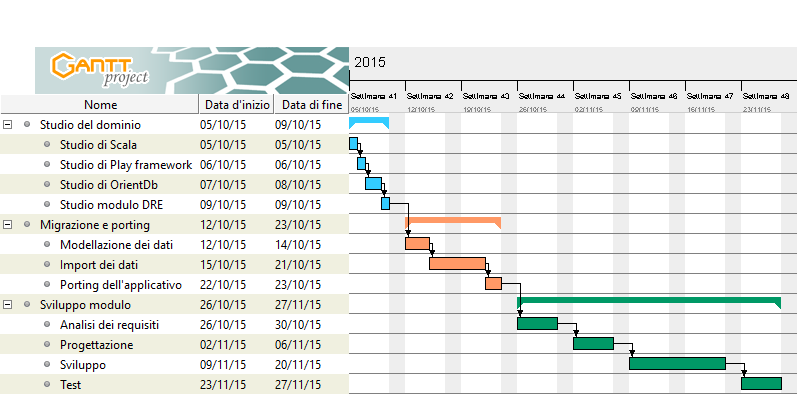
\includegraphics[scale=0.52]{immagini/gantt}
\caption{Suddivisione delle attività}
\label{fig:gantt}
\end{figure}
\newpage
\subsection{Pianificazione}
In sede di pianificazione prima dell'inizio dello \emph{stage} ho programmato 3 macro attività sequenzialmente. Ho assegnato nel primo periodo una settimana per l'attività di studio del dominio, in quanto questa attività è propedeutica alle successive attività. Nel periodo successivo di 2 settimane, ho pianificato l'attività di \emph{porting} dell'applicativo DRE su richiesta del \emph{tutor} aziendale per motivi di strategia aziendale. Nell'ultimo periodo ho programmato l'attività di sviluppo del modulo denominato Tres. Ho privilegiato quest'ultima attività assegnando un totale di 5 settimane lavorative. Qui di seguito illustro le sotto-attività programmate per ogni settimana. 
\begin{itemize}
\item \textbf{Prima settimana:}
\begin{itemize}
\item Studio del \emph{database} OrientDB;
\item Studio del linguaggio di programmazione Scala;
\item Studio del \emph{framework} Play;
\item Studio del progetto preesistente;
\end{itemize}
\item \textbf{Seconda e terza settimana:} migrazione dalla tecnologia MongoDB a OrientDB e \emph{porting} all’ultima versione di Play;
\item \textbf{Quarta settimana:} Analisi dei requisiti del nuovo modulo;
\item \textbf{Quinta settimana:} progettazione architetturale;
\item \textbf{Sesta e settima settimana:} implementazione modulo;
\item \textbf{Ottava settimana:} test.
\end{itemize}
La figura \hyperref[fig:gantt]{3.1} presenta il diagramma di \emph{gantt} utilizzato per la pianificazione.
%**************************************************************




%**************************************************************
\section{Analisi dei requisiti} 
\subsection{Requisiti}
Per l'attività di analisi dei requisiti ho svolto molteplici incontri insieme al \emph{tutor} aziendale per delineare quali funzionalità dovesse offrire il sistema. Il \emph{tutor} mi ha fornito molti esempi ed illustrazioni per capire al meglio quali requisiti il sistema dovesse soddisfare. Una volta definito le funzionalità, ho trascritto i requisiti in un file testuale, in un formato organizzato tabellare. Visto le dimensioni ridotte del progetto ho prediletto il tracciamento dei requisiti con un file di testo anziché utilizzare un sistema automatizzato. Il file è stato poi sottoposto a versionamento all'interno del \emph{repository} per permettere operazioni di consultazione e modifica all'evolversi dei requisiti. La notazione scelta per suddividere i requisiti è la seguente: 
\begin{center}
R[Importanza][Tipologia][Codice]
\end{center}
\begin{itemize}
\item Importanza può assumere i seguenti valori:
\begin{itemize}
\item \textbf{OBB:} requisito obbligatorio. Il soddisfacimento è necessario per il raggiungimento degli obiettivi dello \emph{stage};
\item \textbf{DES:} requisito desiderabile. L'implementazione non è fondamentale, ma dà valore aggiunto al prodotto.
\end{itemize}
\item Tipologia può assumere i seguenti valori:
\begin{itemize}
\item \textbf{F:} requisiti funzionali. Specifica una funzionalità che il \emph{software} deve avere;
\item \textbf{V:} requisiti di vincolo. Specifica il vincolo che il \emph{software} deve avere;
\item \textbf{P:} requisiti di prestazione. Specifica un vincolo di \emph{performance} che il \emph{software} deve fornire.
\end{itemize}
\item Codice è un \emph{id} numerico univoco.
\end{itemize}
\newpage
Tabella requisiti:
\def\arraystretch{1.8}
\begin{longtable}{|l|p{7cm}|}
\hline
\textbf{Codice} &	\textbf{Descrizione}	\\\hline
ROBBF1	&	Il sistema deve permettere l'inserimento di un nuovo comportamento	\\\hline
ROBBF2	&	Il sistema deve restituire un messaggio di segnalazione in caso di errore durante il salvataggio \\\hline
ROBBF3	&	I dati ricevuti devono essere in formato Json \\\hline
ROBBF4	&	I dati inviati devono essere in formato Json \\\hline
ROBBF5	&	Il sistema deve restituire un messaggio di errore in caso di Json non valido \\\hline
ROBBF6	&	Devono essere inseriti almeno 100 comportamenti per produrre la raccomandazione \\\hline
ROBBF7	&	Il sistema deve restituire un messaggio di conferma quando l'algoritmo è pronto a produrre una raccomandazione	\\\hline
ROBBF8	&	Il sistema deve permettere il calcolo dell'entropia del \emph{dataset} \\\hline
ROBBF9	&	Il sistema deve permettere il calcolo del guadagno di informazione del \emph{dataset}	\\\hline
ROBBV10	&	Il sistema deve permettere la costruzione ricorsivamente dell'albero di decisione	\\\hline
ROBBV11	&	Il sistema deve permettere la creazione di tanti nodi quanti sono i possibili valori dell'attributo scelto \\\hline
ROBBV12	&	L'algoritmo di costruzione dell'albero deve fermarsi quando tutte le istanze di un nodo appartengono alla stessa classe \\\hline
ROBBF13	&	Il sistema deve permettere di ricevere una richiesta per classificare un comportamento vuoto \\\hline
ROBBF14	&	Il sistema, per la richiesta con un comportamento vuoto, deve restituire tutte le raccomandazioni con le percentuale calcolate in base al \emph{dataset} \\\hline
ROBBF15	&	Il sistema deve permettere di classificare un comportamento dell'utente \\\hline
ROBBF16	&	Il sistema deve fornire una raccomandazione o più in base alla classificazione del comportamento \\\hline
ROBBF17	&	Il sistema deve fornire insieme alla raccomandazione la percentuale di adeguatezza	\\\hline
ROBBV18	&	Il sistema deve permettere la modifica dell'albero di decisione ogni 24 ore	\\\hline
ROBBV19	&	Devono essere rispettate le metriche sulla stesura del codice riportate nella sezione 3.5 \\\hline
RDESF20	&	Devono essere implementati nuovi algoritmi basati sulla teoria de giochi	\\\hline
RDESV21	&	Devono essere implementati nuovi algoritmi di \emph{clustering}	\\\hline
RDESV22	&	Deve essere sviluppato il pannello di amministrazione	\\\hline
ROBBP23	&	Il \emph{database} deve essere in grado di memorizzare almeno 100.000 record al secondo	\\\hline
\caption{Tabella dei requisiti}
\end{longtable}
\subsection{Casi d'uso}
Durante l'analisi dei requisiti ho realizzato dei diagrammi \emph{UML}, utilizzando il \emph{software} Astah. Tres è concepito per operare con Bdrim, una piattaforma di raccolta dati sviluppato in collaborazione con Allos. Quindi l'unico attore coinvolto nell'utilizzo di Tres è Bdrim che espone un caso d'uso principale. In questa sezione riporto i casi d'uso principali che descrivono maggiormente il sistema nel suo complesso. Per ogni caso d'uso ho specificato: 
\begin{itemize}
\item Gli attori coinvolti;
\item Pre e post condizione;
\item Scopo e descrizione;
\item Flusso principale degli eventi.
\end{itemize}
Inoltre, se previsto, ho specificato estensione e lo scenario alternativo.
\newpage
\subsubsection{UC0}
\begin{figure}[h]
\centering
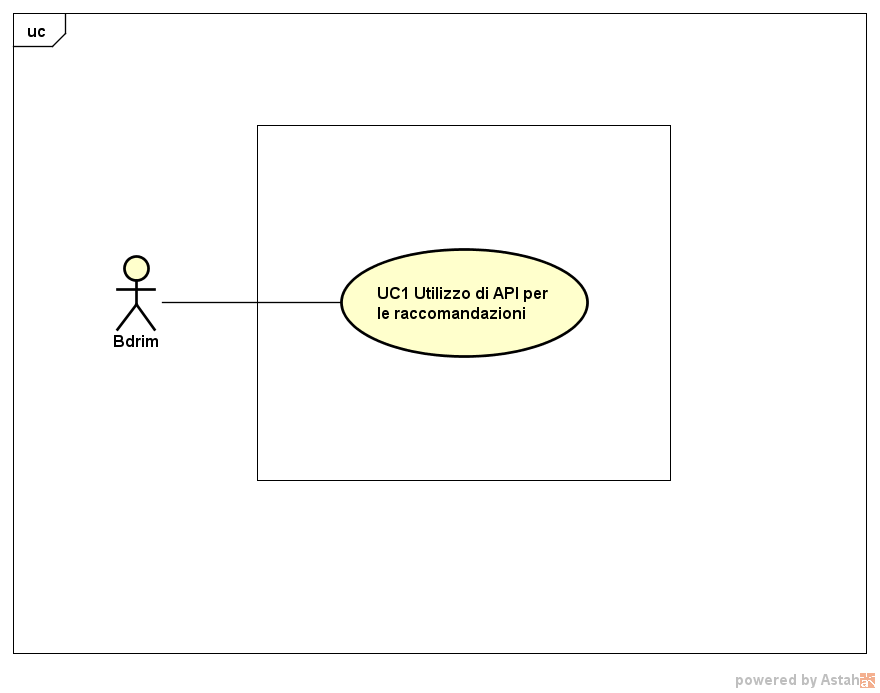
\includegraphics[scale=0.42]{immagini/UC0a}
\caption{UC0: Tres}
\label{fig:UC0}
\end{figure}
\begin{itemize}
\item \textbf{Attori:} Bdrim
\item \textbf{Scopo e descrizione:} Questo caso d'uso descrive le funzionalità messe a disposizione dal sistema. Principalmente Bdrim può usufruire delle \emph{API} per le raccomandazioni fornite da Tres.
\item \textbf{Pre-condizione:} Il \emph{server} è stato avviato.
\item \textbf{Flusso principale degli eventi:} Bdrim utilizza le \emph{API} per ottenere una raccomandazione.
\item \textbf{Post-condizione:} Il sistema risponde alle richieste HTTP effettuata da Bdrim.
\end{itemize}
\newpage
\subsubsection{UC1}
\begin{figure}[h]
\centering
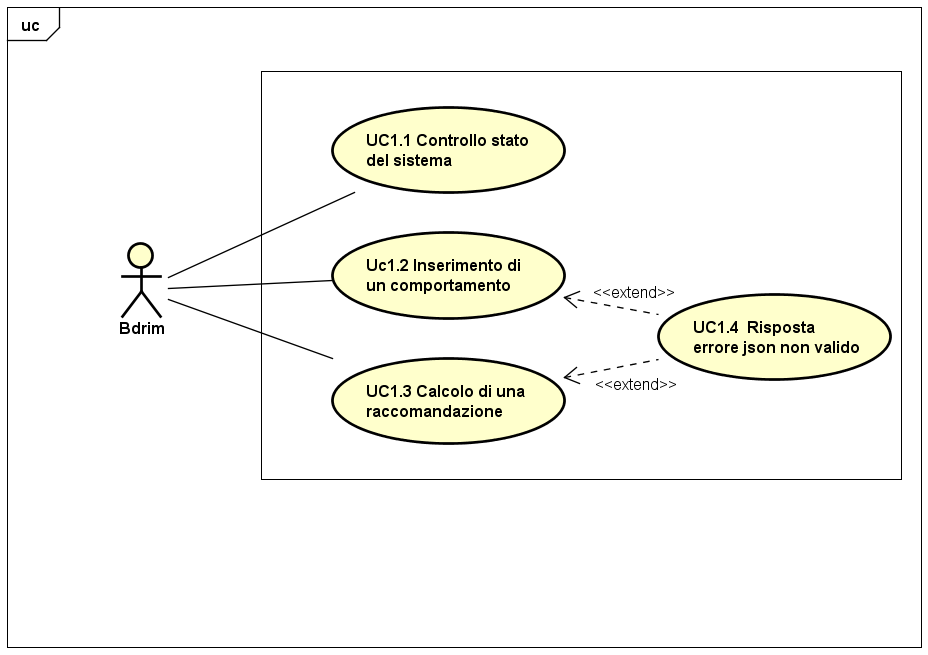
\includegraphics[scale=0.42]{immagini/UC1a}
\caption{UC1: Tres}
\label{fig:UC1}
\end{figure}
\begin{itemize}
\item \textbf{Attori:} Bdrim
\item \textbf{Scopo e descrizione:} Questo caso d'uso illustra le funzionalità offerte dal sistema a Bdrim. Bdrim ha la possibilità di effettuare delle richieste \emph{REST} al sistema;
\item \textbf{Pre-condizione:} Il \emph{server} è stato avviato e Tres è stato attivato.
\item \textbf{Flusso principale degli eventi:}
\begin{itemize}
\item[1] Bdrim richiede lo stato del sistema [UC1.1];
\item[2] Nel caso il sistema sia pronto Bdrim richiede la raccomandazione[UC1.3];
\item[3] Bdrim può inserire un comportamento[UC1.2].
\end{itemize}
\item \textbf{Scenario alternativo:} Bdrim effettua delle richieste \emph{HTTP} inviando un oggetto \emph{Json} malformato oppure invalido e ritorna una risposta \emph{HTTP} che segnala l'errore in formato \emph{Json}. 
\item \textbf{Estensione:} Bdrim riceve una risposta \emph{HTTP} e all'interno il \emph{Json} che segnala l'errore di dati non validi [UC1.4];
\item \textbf{Post-condizione:} Il sistema risponde alle richieste \emph{HTTP} ritornando una risposta \emph{HTTP}, ritornando i dati in formato \emph{Json}.
\end{itemize}
%**************************************************************




%**************************************************************
\newpage
\section{Progettazione architetturale}
Questa sezione descrive l'attività di progettazione. Illustra l'architettura generale del sistema, le relazioni interne, la struttura del \emph{database} e infine i \emph{design pattern} utilizzati.
\subsection{Visione ad alto livello}
Il contesto di utilizzo dell'applicativo è la piattaforma di Bdrim. Questa piattaforma permette di gestire nuovi moduli per introdurre nuove funzionalità. Ogni modulo deve essere assolutamente isolato per poter essere facilmente modificabile e interscambiabile con altri moduli che migliorino le sue funzionalità. Quindi la visione generale del sistema si riconduce ad un modello \emph{client-server} dove i ruoli sono:
\begin{itemize}
\item \textbf{Server:} rappresentato da Tres, elabora le richieste \emph{HTTP} ricevute da Bdrim.
\item \textbf{Client:} rappresentato unicamente da Bdrim.
\end{itemize}
%\begin{figure}[h]
%\centering
%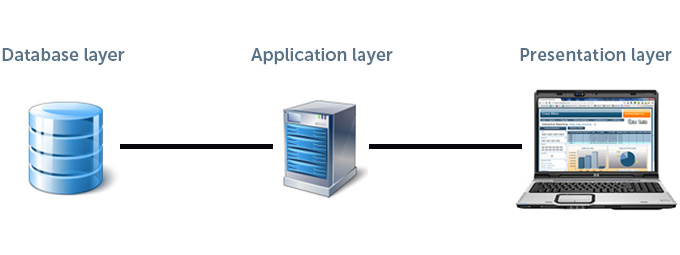
\includegraphics[scale=0.42]{immagini/client-server}
%\caption{Visione generale architettura \emph{client-server}. Immagine tratta da \href{http://%contentdeliverance.com/2011/client-server-architecture/}{Content Deliverance}}
%\label{fig:client-server}
%\end{figure}
\begin{figure}[h]
\centering
\includegraphics[scale=0.50]{immagini/architetturagenerale}
\caption{Visione generale dell'architettura}
\label{fig:arch-gen}
\end{figure}
Le due componenti sono indipendenti tra loro e comunicano utilizzando una architettura \emph{REST}.
\newpage
\subsection{Architettura}
Per la realizzazione di Tres, ho seguito un \emph{design} architetturale \emph{MVC}. Quindi i \emph{package} principali sono \emph{model}, \emph{view} e \emph{controller}. Attualmente il \emph{package} \emph{views} non viene utilizzato, il suo utilizzo tornerà utile in eventuali sviluppi successivi per la creazione di una interfaccia di amministrazione per Bdrim o altre eventuali funzionalità. Qui di seguito illustro la visione generale e successivamente le componenti del sistema.  
\begin{figure}[h]
\centering
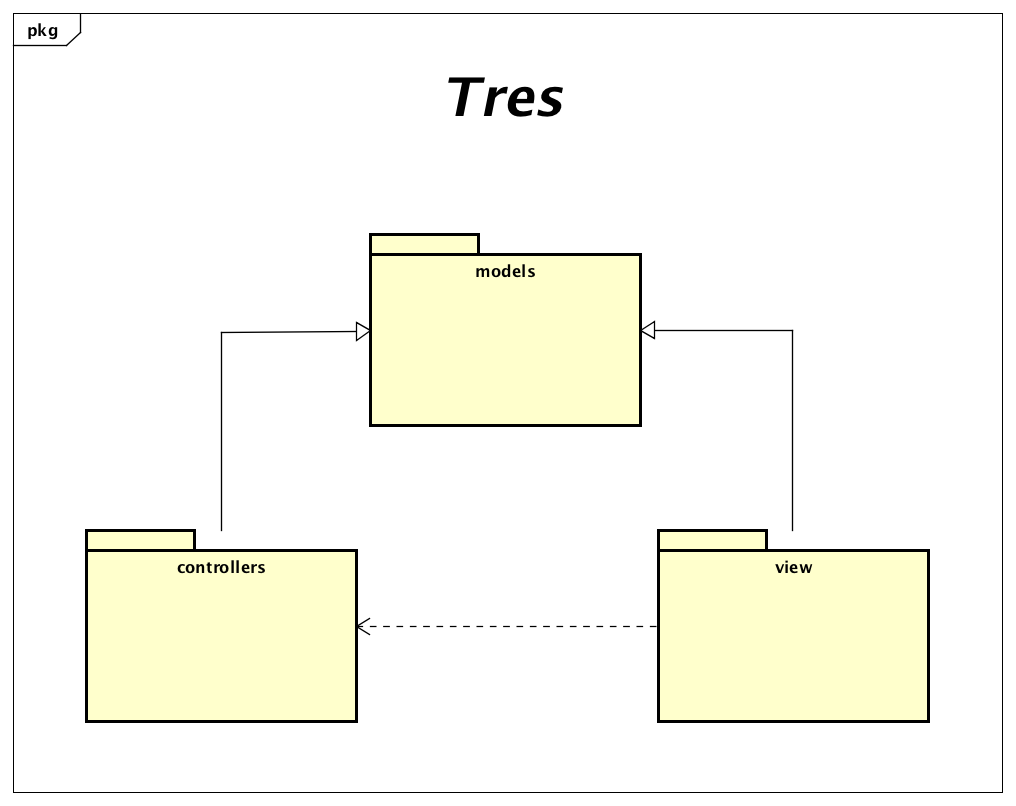
\includegraphics[scale=0.35]{immagini/architetturamvc}
\caption{Visione generale dell'architettura}
\label{fig:arch-gen}
\end{figure}
\newpage
\subsubsection{controllers}%procedere da qui
Il \emph{package} \emph{controllers} contiene le componenti responsabili della logica di controllo e nello specifico contiene due classi. \emph{BridgeController} è la componente che gestisce le richieste \emph{HTTP} instradate dalla componente \emph{router} del \emph{framework} Play. Il \emph{package} interagisce con \emph{model} utilizzando i servizi messi a disposizione e le rappresentazioni dei dati.
\begin{figure}[h]
\centering
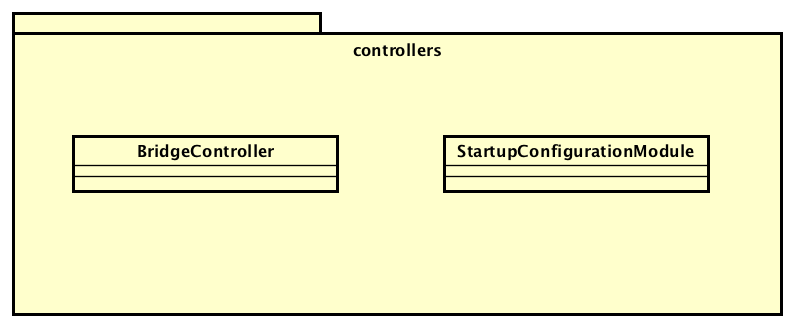
\includegraphics[scale=0.35]{immagini/controllers}
\caption{Diagramma del \emph{package} \emph{controllers}}
\label{fig:pack-controller}
\end{figure}
\subsubsection{models}
Il \emph{package} \emph{models} contiene tutta la logica di \emph{business} del sistema e di accesso ai dati. E' responsabile di fornire una separazione dalla rappresentazione interna dei dati del database. Fornisce tutte le interfacce necessarie al \emph{controller} necessarie per fornire i servizi.
\begin{figure}[h]
\centering
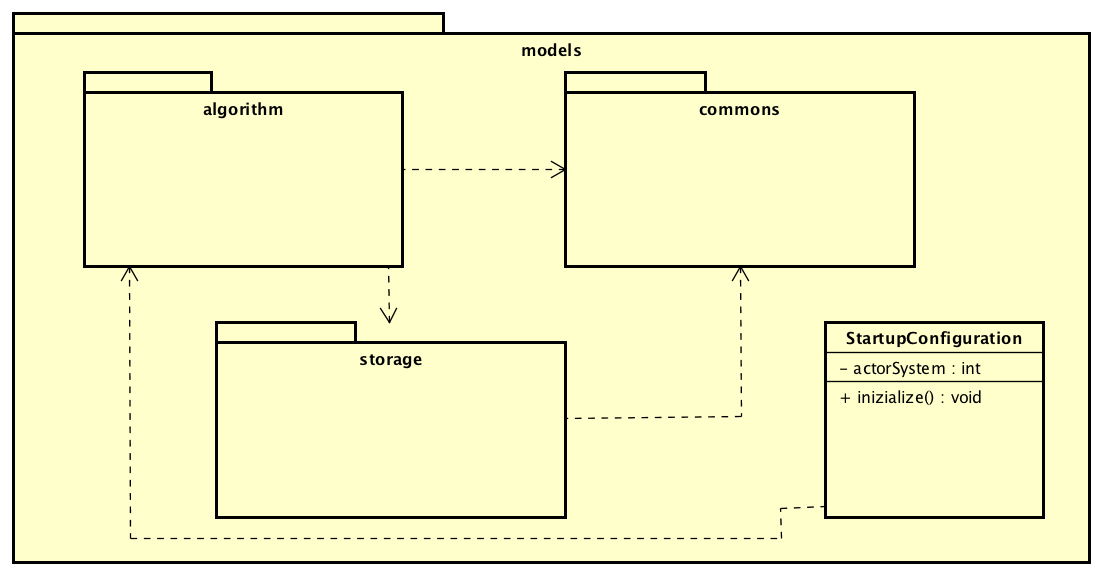
\includegraphics[scale=0.30]{immagini/models}
\caption{Diagramma del \emph{package} \emph{models}}
\label{fig:pack-models}
\end{figure}
\paragraph{Classi contenute}
\begin{itemize}
\item \textbf{StartupConfiguration:} Questa classe è responsabile di schedulare la generazione dell'albero per le raccomandazioni. La generazione dell'albero avviene ogni 24 ore e solamente se sono disponibili almeno 100 comportamenti memorizzati.
\end{itemize}
\paragraph{Package contenuti}
\paragraph*{commons}
Il \emph{package} \emph{commons} contiene le componenti per la rappresentazione interna dei dati. All'interno sono presenti dei convertitori impliciti, che permettono la validazione e la conversione in formato Json, funzionalità utili per le componenti nel \emph{controller}. 
\begin{figure}[h]
\centering
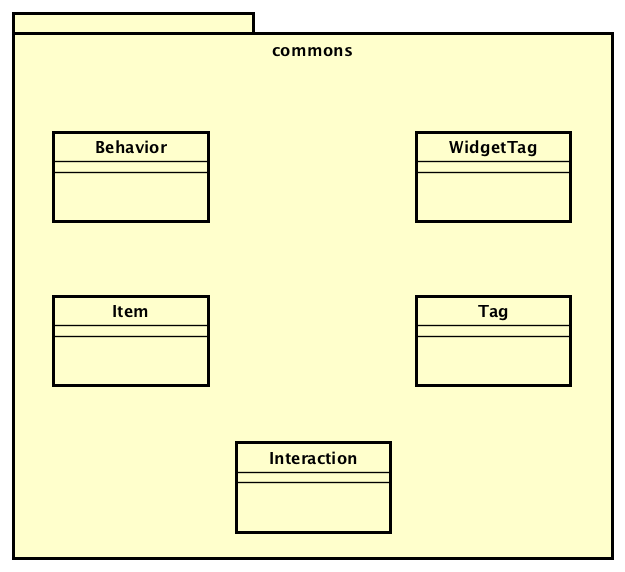
\includegraphics[scale=0.28]{immagini/commons}
\caption{Diagramma del \emph{package} \emph{commons}}
\label{fig:pack-commons}
\end{figure}
\paragraph*{storage}
Il \emph{package} \emph{storage} è responsabile dell'accesso ai dati. Fornisce una interfaccia che fornisce delle funzionalità \emph{CRUD}. Il \emph{package} dipende dalle componenti in \emph{commons}, e per ognuna implementa l'interfaccia per l'interazione con OrientDb. Le componenti che gestiscono la persistenza in OrientDb utilizzano le API Blueprints\footcite{https://github.com/tinkerpop/blueprints} perchè OrientDb aderisce a questo standard di default. TinkerPop Blueprints fornisce delle API per manipolare \emph{database} a grafo ed è incluso nello \emph{stack} dei progetti di TinkerPop\footcite{http://tinkerpop.incubator.apache.org/}
\begin{figure}[h]
\centering
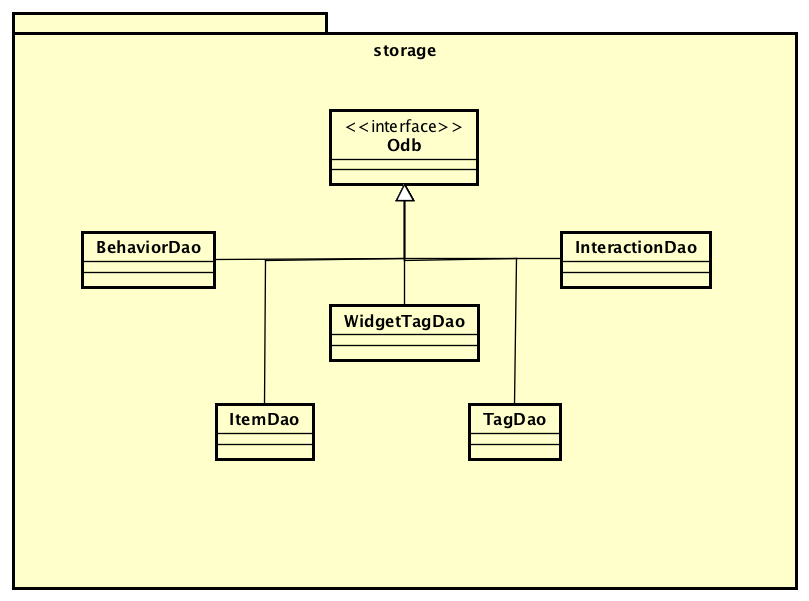
\includegraphics[scale=0.28]{immagini/storage}
\caption{Diagramma del \emph{package} \emph{storage}}
\label{fig:pack-storage}
\end{figure}
\newpage
\paragraph*{algorithm}
Il \emph{package} \emph{algorithm} contiene le componenti \emph{software} che realizzano l'algoritmica basata essenzialmente su \emph{ID3} ed è fortemente dipendente dalle componenti presenti in \emph{commons}. Fornisce la funzionalità per la costruzione dell'albero decisionale sulla base dei \emph{behavior} in \emph{input}. Offre la funzionalità per ricevere in \emph{output} la raccomandazione sulla base di un \emph{behavior} in \emph{input}.
\begin{figure}[h]
\centering
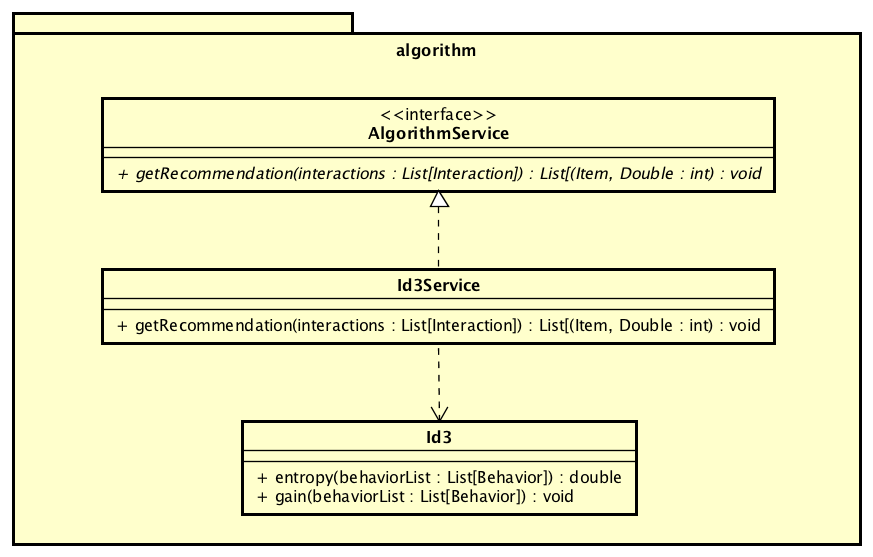
\includegraphics[scale=0.30]{immagini/algorithm}
\caption{Diagramma del \emph{package} \emph{algorithm}}
\label{fig:pack-algorithm}
\end{figure}
\subsection{Database}
OrientDb è un \emph{database} a grafo, quindi esistono due entità, i vertici e gli spigoli. Entrambi possono contenere degli attributi al loro interno, ma nel caso degli spigoli è fortemente sconsigliato per motivi prestazionali\footnote{http://orientdb.com/docs/last/Performance-Tuning-Graph.html}. Per la persistenza dei dati ho scelto una definizione dei dati di tipo \emph{schema-full} per evitare un controllo dei dati a \emph{run-time} nelle componenti del \emph{package} \emph{storage}.\\
Il vertice principale è \emph{Behavior} che rappresenta il comportamento di un utente. Da un \emph{behavior} si dirama l'associazione verso un \emph{Item} attraverso lo spigolo \emph{Result} ed esprime che il comportamento dell'utente ha come risultato un \emph{Item}. Un \emph{Item} è descritto con una serie di \emph{Tag}, quindi un vertice di tipo \emph{Item} è associato a molteplici \emph{Tag} tramite uno spigolo \emph{HoldsTag}. Un \emph{Behavior} descrive una serie di interazioni su dei \emph{WidgetTag}, quindi un vertice di tipo \emph{Behavior} è associato a molteplici \emph{WidgetTag} tramite uno spigolo \emph{Interaction}. \emph{Interaction} contiene la tipologia svolta su di un determinato \emph{WidgetTag}.
\begin{figure}[h]
\centering
\includegraphics[scale=0.45]{immagini/databaseschema}
\caption{Diagramma del \emph{package} \emph{algorithm}}
\label{fig:pack-algorithm}
\end{figure}
\subsection{Design pattern}
Qui di seguito elenco i \emph{design pattern} utilizzati per la realizzazione di Tres.
\subsubsection{MVC}
\begin{figure}[h]
\centering
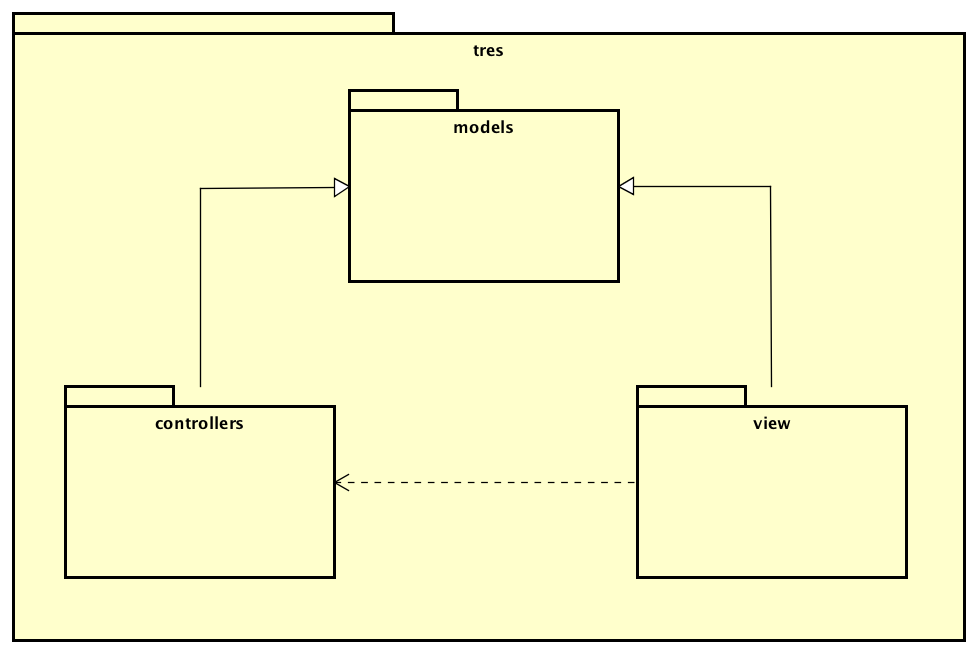
\includegraphics[scale=0.20]{immagini/mvc}
\caption{Contesto di utilizzo del \emph{design pattern MVC}}
\label{fig:pattern-mvc}
\end{figure}
\begin{itemize}
\item\textbf{Scopo dell'utilizzo:} questo \emph{design pattern} viene utilizzato per separare i compiti delle diverse componenti \emph{software} dell'applicazione, separando \emph{business logic}, \emph{application logic} e viste, rappresentate rispettivamente da \emph{models}, \emph{controller} e \emph{views};
\item \textbf{Contesto di utilizzo:} questo \emph{pattern} viene implementato nativamente dal \emph{framework} Play. In particolare implementa una tipologia di \emph{MVC pull-model} che permette un salto tecnologico tra la \emph{view} e il \emph{controller}.
\end{itemize}
\subsubsection{Dao}
\begin{figure}[h]
\centering
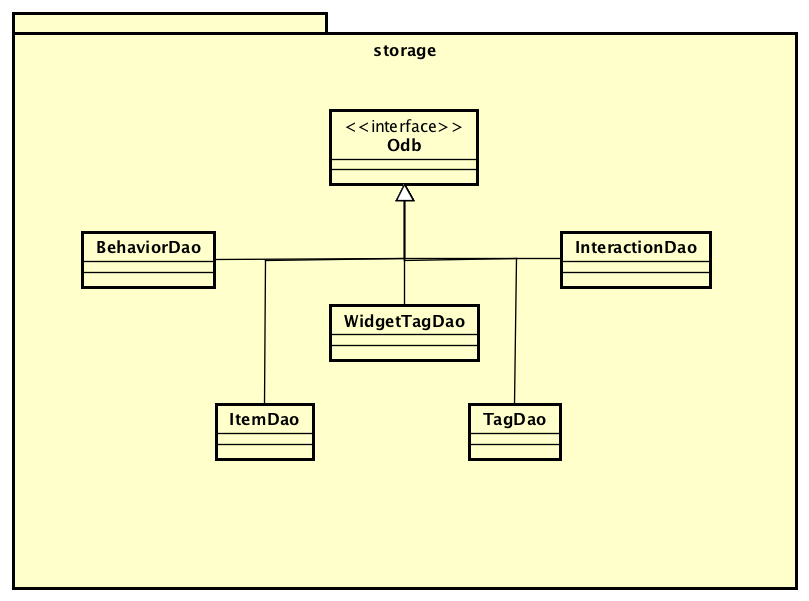
\includegraphics[scale=0.20]{immagini/storage}
\caption{Contesto di utilizzo del \emph{design pattern DAO}}
\label{fig:pattern-dao}
\end{figure}
\begin{itemize}
\item\textbf{Scopo dell'utilizzo:} questo \emph{design pattern} è utilizzato per disaccoppiare la logica di \emph{business} dalla logica di persistenza. Per rendere così le componenti indipendenti dal sistema di \emph{database};
\item \textbf{Contesto di utilizzo:} viene utilizzato dalle componenti presenti nel \emph{package storage} per interagire col \emph{database} OrientDb.
\end{itemize}
\subsubsection{Strategy}
\begin{figure}[h]
\centering
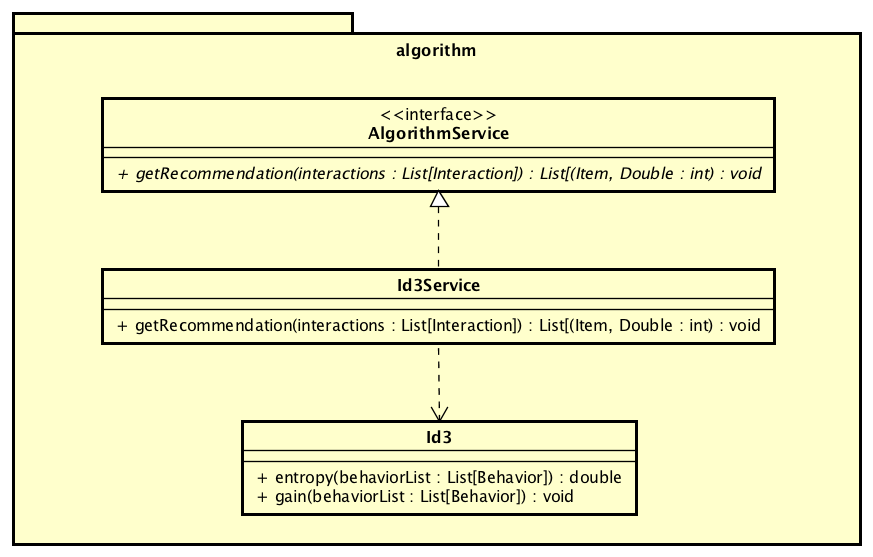
\includegraphics[scale=0.30]{immagini/algorithm}
\caption{Contesto di utilizzo del \emph{design pattern strategy}}
\label{fig:pattern-strategy}
\end{figure}
\begin{itemize}
\item\textbf{Scopo dell'utilizzo:} il \emph{design pattern strategy} definisce una famiglia di algoritmi, incapsulati e resi intercambiabili. \emph{Strategy} permette agli algoritmi di variare indipendentemente dai client che ne fanno uso;
\item \textbf{Contesto di utilizzo:} viene utilizzato dalle componenti presenti nel \emph{package algorithm}. E' presente una interfaccia per l'algoritmo che viene implementata da \emph{Id3Service}, che realizza l'algoritmo \emph{ID3}.
\end{itemize}
\subsubsection{Singleton}
\begin{figure}[h]
\centering
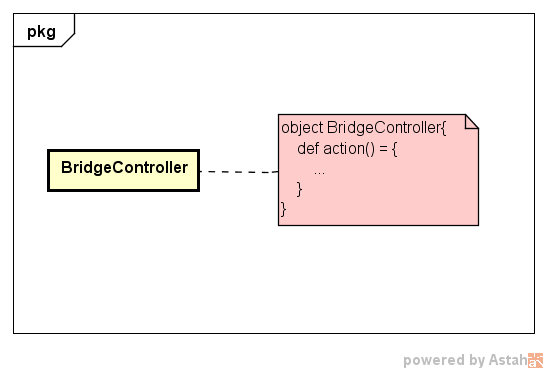
\includegraphics[scale=0.50]{immagini/singleton}
\caption{Contesto di utilizzo del \emph{design pattern singleton}}
\label{fig:pattern-singleton}
\end{figure}
\begin{itemize}
\item\textbf{Scopo dell'utilizzo:} il \emph{design pattern singleton} assicura che una certa classe abbia una sola istanza e fornisce un punto d'acceso globale a tale istanza;
\item \textbf{Contesto di utilizzo:} viene utilizzato nelle componenti del \emph{package controller} e viene implementato nativamente dal linguaggio Scala dichiarando la classe come \emph{object}.
\end{itemize}
%**************************************************************



%**************************************************************
\newpage
\section{Progettazione di dettaglio}
La progettazione di dettaglio con la metodologia \emph{agile} avviene di pari passo durante la codifica, il che è rischioso perché introduce molti errori di codifica, tuttavia le ore risparmiate della progettazione di dettaglio sono state reimpiegate nel correggere eventuali errori. Riporto qui di seguito i diagrammi di sequenza UML più significativi:
\subsection{Controllo stato}
In fase di \emph{startup} il sistema non possiede nessun dato, e quindi non è in grado di fornire raccomandazioni. Un modo per verificare lo stato operativo del modulo è attraverso una chiamata mediante questa chiamata dell'interfaccia \emph{REST}:\\
\def\arraystretch{1.5}
\begin{longtable}{|p{2.5cm}|p{5cm}|l|}
\hline
\textbf{Tipo} &	\textbf{Chiamata}	\\\hline
GET		&	/tres/ready		 \\\hline
\end{longtable}
\begin{figure}[h]
\centering
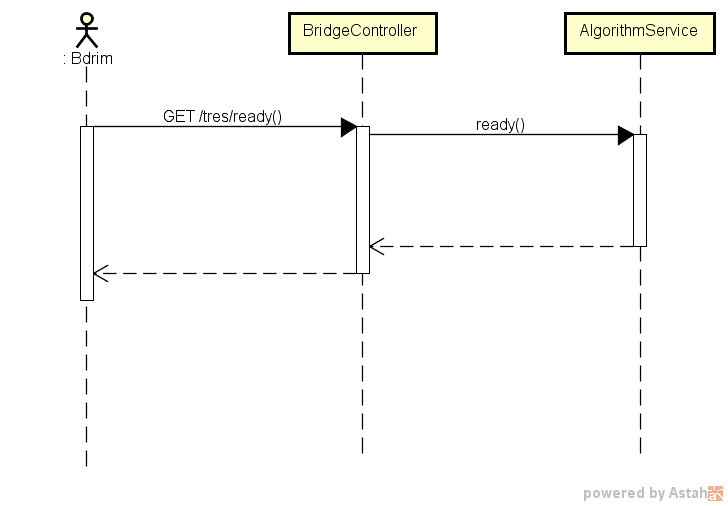
\includegraphics[scale=0.43]{immagini/DScheckstate}
\caption{Diagramma di sequenza: controllo stato.}
\label{fig:seq-controllostato}
\end{figure}
Mediante il \emph{router} la richiesta \emph{HTTP} giunge fino ad al metodo \emph{ready} della classe \emph{BridgeController} che a sua volta controllerà la presenza dell'albero tramite \emph{AlgorithmService}. Al termine ritorna in \emph{output} una risposta \emph{HTTP} contenente un oggetto \emph{Json}.

\subsection{Inserimento behavior}
Per istruire l'algoritmo di selezione è necessario fornire dei dati per l'apprendimento. Ho implementato una procedura di inserimento dei comportamenti mediante questa chiamata dell'interfaccia \emph{REST}:
\def\arraystretch{1.5}
\begin{longtable}{|p{2.5cm}|p{5cm}|l|}
\hline
\textbf{Tipo} &	\textbf{Chiamata}	\\\hline
POST	&	/tres/behavior	 \\\hline
\end{longtable}
\begin{figure}[h]
\centering
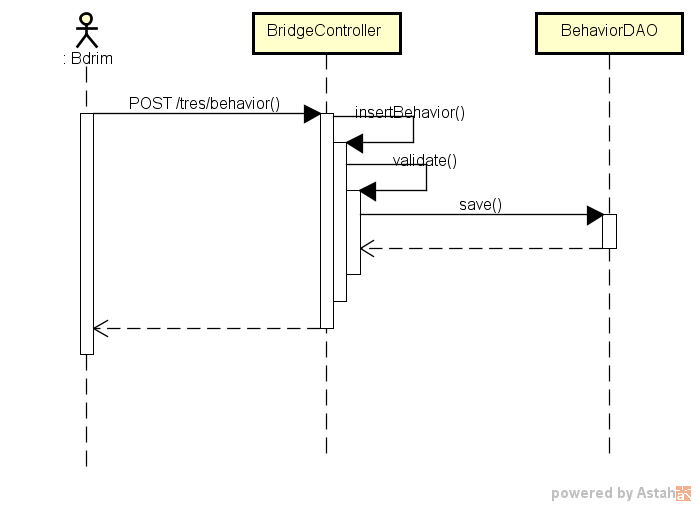
\includegraphics[scale=0.42]{immagini/DSinsertBeh}
\caption{Diagramma di sequenza: inserimento comportamento.}
\label{fig:seq-inserimentobeh}
\end{figure}
Da Bdrim arriva una richiesta \emph{HTTP POST} che comprende un \emph{Json} contenente un \emph{Behavior}. Il \emph{router} di Play accoglie la richiesta che la reindirizza al metodo della classe \emph{BridgeController insertBehavior}. Il flusso continua con la validazione del \emph{Json} e successivamente inserisce il comportamento invocando il metodo \emph{save} della classe \emph{BehaviorDAO}. 


\subsection{Raccomandazione}
Una volta raccolti almeno 100 \emph{Behavior} e che l'algoritmo ha generato l'albero, il sistema è in grado di fornire una raccomandazione. Ho implementato la procedura di raccomandazione mediante questa chiamata dell'interfaccia REST:
\def\arraystretch{1.5}
\begin{longtable}{|p{2.5cm}|p{5cm}|l|}
\hline
\textbf{Tipo} &	\textbf{Chiamata}	\\\hline
POST	&	/tres/recommendation	 \\\hline
\end{longtable}
\begin{figure}[h]
\centering
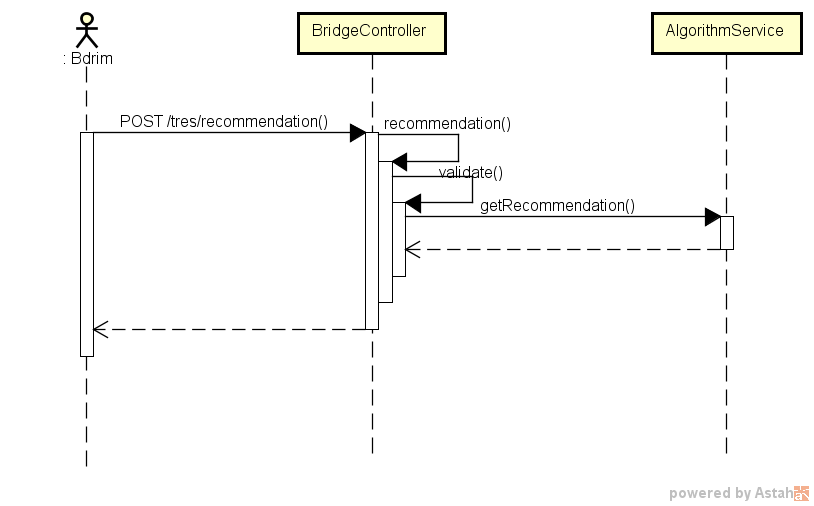
\includegraphics[scale=0.42]{immagini/DSracommandazione}
\caption{Diagramma di sequenza: raccomandazione.}
\label{fig:seq-inserimentobeh}
\end{figure}
Da Bdrim arriva una richiesta \emph{HTTP POST} che comprende un \emph{Json} contenente le interazioni dell'utente. Il \emph{router} convoglia la richiesta al metodo \emph{recommendation} di \emph{BridgeController}. Il flusso procede con la validazione del \emph{Json} ricevuto che estrapola una lista di interazioni dell'utente. Questa lista viene elaborata dall'albero tramite la chiamata al metodo \emph{getRecommendation} di \emph{AlgorithmService} che ritornerà le probabilità delle raccomandazioni. 
%**************************************************************




%**************************************************************
\newpage
\section{Verifica e Validazione}
Questa sezione descrive l'attività di verifica e validazione svolta durante la realizzazione di Tres, indicando gli strumenti utilizzati utilizzati, le metriche utilizzate e infine un resoconto finale dei test. L'attività di verifica mi ha permesso di individuare prontamente errori di codifica e ridurre i tempi di sviluppo. Ho cercato di automatizzare il più possibile questa attività per focalizzarmi nello sviluppo. In primis ho effettuato dei test di unità per le componenti più complesse e successivamente ho verificato la loro integrazione. Per motivi di tempo non ho potuto realizzare tutti test di unità e di integrazione per tutte le componenti, mi sono focalizzato sulle componenti principali. 
\subsubsection{Strumenti}
Durante lo sviluppo ho utilizzato il più possibile degli automatismi che mi permettessero di fare analisi statica e dinamica risparmiando più tempo possibile. Ho adottato i seguenti strumenti:
\begin{itemize}
\item \textbf{Intellij IDEA:} questo IDE fornisce funzionalità per identificare errori di programmazione come ad esempio sintassi errata, incompatibilità tra tipi e variabili non definite. Fornisce la percentuale di documentazione dell'intero progetto.
\item \textbf{TravisCI:} è uno strumento che fornisce un automatismo per la compilazione e l'esecuzione dei \emph{test} del progetto. Se la compilazione o almeno un test fallisce, invia una notifica via \emph{email} con la possibilità di consultare il \emph{log}.
\item \textbf{Codecov:} questo strumento fornisce la percentuale delle linee di codice coperte durante i \emph{test}.
\item \textbf{Specs2:} è una libreria di \emph{testing} fornita direttamente da Play Framework. Mi ha permesso di testare l'intera applicazione anche con le chiamate HTTP.
\end{itemize}
\subsubsection{Metriche adottate}
Per la realizzazione di Tres ho adottato le seguenti metriche:
\begin{itemize}
\item \textbf{Attributi per classe:}  un numero troppo elevato di attributi potrebbe indicare la necessità di suddividere la classe in una gerarchia. Ho fissato un \emph{range} ottimale i seguenti valori, un minimo 1 fino ad un massimo di 8;
\item \textbf{Complessità ciclomatica:} è un indice utilizzato per misurare la complessità di funzioni, metodi, moduli e classi di un programma. Misura direttamente il numero di cammini linearmente indipendenti attraverso il grafo di controllo di flusso. I nodi del grafo corrispondono a gruppi indivisibili di istruzioni, mentre gli archi connettono due nodi se il secondo gruppo di istruzioni può essere eseguito immediatamente dopo il primo gruppo. Per questa metrica ho fissato un \textit{range} ottimale da un minimo di 1 fino ad un massimo di 10;
\newpage
\item \textbf{Copertura dei commenti:} è indice della percentuale di classi e metodi corredati di commenti. Ho fissato un range ottimale da 80\% a 100\%;
\item \textbf{Copertura dei test:} è una metrica utilizzata per misurare l'efficacia del collaudo. Si utilizza un indice che tiene traccia di quante volte è stata eseguita ogni istruzione durante il \emph{testing}, le istruzioni eseguite almeno una volta sono dette "coperte". L'obiettivo è coprire il maggior numero possibile di istruzioni, in modo da avere una minore quantità di errore. Per questa metrica ho fissato un valore ottimale minimo di 70\%.
\end{itemize}
\subsection{Resoconto risultati}
\subsubsection{Metriche misurate}
Qui di seguito sono riportate le metriche software misurate:
\begin{itemize}
\item \textbf{Complessità ciclomatica:} per il calcolo della complessità ciclomatica ho utilizzato Sbt, al suo interno è disponibile il \emph{tool} styleCheck. Questo strumento segnala con un \emph{warning} se la complessità supera il valore 10. Il \emph{tool} ha restituito esito positivo e non ha segnalato alcun \emph{warning};
\item \textbf{Attributi per classe:} ho rilevato per questa metrica come valore medio 2, mentre come valore massimo ho rilevato 4;
\item \textbf{Copertura commenti:} il valore di copertura è pari al 100\%;
\item \textbf{Copertura dei test:} il valore di copertura dei \emph{test} è del 73\%.
\end{itemize}
\subsubsection{Test di unità}
Qui di seguito sono riportati tutti i \emph{test} di unità eseguiti e il loro relativo esito:
\def\arraystretch{1.8}
\begin{longtable}{|l|p{7cm}|l|}
\hline
\textbf{Test} &	\textbf{Descrizione}	&	\textbf{Stato}	\\\hline
TU1	&	Viene verificato che il sistema salvi correttamente un comportamento all'interno del \emph{database}	&	Esito positivo	\\\hline
TU2	&	Viene verificato il corretto caricamento di una lista di \emph{widgetTag} distinti	&	Esito positivo	\\\hline
TU3	&	Viene verificato il corretto caricamento di una lista di \emph{item} distinti	&	Esito positivo	\\\hline
TU4	&	Viene verificato il corretto caricamento di una lista di \emph{behavior} con una \emph{interaction} specifica	&	Esito positivo	\\\hline
TU5	&	Viene verificato il corretto caricamento di una lista di \emph{behavior} con \emph{tag} e \emph{action} specifici	&	Esito positivo	\\\hline
TU6	&	Viene verificato il corretto caricamento di una lista di \emph{action} distinti	&	Esito positivo	\\\hline
TU7	&	Viene verificato il corretto calcolo dell'entropia	&	Esito positivo	\\\hline
TU8	&	Viene verificato il corretto calcolo del guadagno di informazione	&	Esito positivo	\\\hline
TU9	&	Viene verificato che venga creata la raccomandazione corretta da fornire	&	Esito positivo	\\\hline
TU10	&	Viene verificato il corretto calcolo delle probabilità	&	Esito positivo	\\\hline
\caption{Tabella dei \emph{test} di unità}
\end{longtable}
\subsubsection{Test di integrazione}
Qui di seguito sono riportati tutti i \emph{test} di integrazione eseguiti e il loro relativo esito:
\def\arraystretch{1.8}
\begin{longtable}{|l|p{7cm}|l|l|}
\hline
\textbf{Test} &	\textbf{Descrizione}	&	\textbf{Componente}	&	\textbf{Stato}	\\\hline
TI1	&	Viene verificato che il sistema crei correttamente un albero di decisione	&	algorithm	&	Esito positivo	\\\hline
TI2	&	Viene verificato che il sistema aggiorni l'albero di decisione ogni 24 ore	&	algorithm	&	Esito positivo	\\\hline
TI3	&	Viene verificata la corretta creazione del \emph{training set}		&	algorithm	&	Esito positivo	\\\hline
\caption{Tabella dei \emph{test} di integrazione}
\end{longtable}
\subsubsection{Test di sistema}
Ho effettuato alcuni \emph{test} di sistema inerenti alle funzionalità di inserimento dati, calcolo di una raccomandazione e infine il calcolo probabilità.
\begin{itemize}
\item \textbf{Inserimento dati:} viene verificato il corretto comportamento del sistema alla richiesta di inserimento dati;
\item \textbf{Calcolo raccomandazioni:} viene verificato il calcolo della raccomandazione da fornire;
\item \textbf{Calcolo probabilità:} viene verificato il calcolo delle probabilità associate ai vari \emph{item}.
\end{itemize}
\subsubsection{Sommario funzionamento}
TODO
%**************************************************************
